\documentclass[prl,twocolumn]{revtex4-1}

\usepackage{graphicx}
\usepackage{color}
\usepackage{latexsym,amsmath}
\usepackage{comment}
\usepackage{tabularx}
\usepackage{siunitx}
\usepackage{multirow}
\usepackage{mathtools}
\usepackage{tikz, fp}
\usepackage{wrapfig}
\usepackage{amsfonts}


\usetikzlibrary{matrix,positioning,fit,backgrounds,intersections}

\usetikzlibrary{calc}

%%%%%%%%%%%%%%%%%%%%%%%%%%%%%%%%%%%%%%%%%%%%%%%%%%%%%%%%%%
%%%%%%%%%%%%%%%%%%%%%%%%%%%%%%%%%%%%%%%%%%%%%%%%%%%%%%%%%%
% DO NOT TOUCH. IT'S DANGEROUS
\makeatletter
\def\calcLength(#1,#2)#3{%
\pgfpointdiff{\pgfpointanchor{#1}{center}}%
             {\pgfpointanchor{#2}{center}}%
\pgf@xa=\pgf@x%
\pgf@ya=\pgf@y%
\FPeval\@temp@a{\pgfmath@tonumber{\pgf@xa}}%
\FPeval\@temp@b{\pgfmath@tonumber{\pgf@ya}}%
\FPeval\@temp@sum{(\@temp@a*\@temp@a+\@temp@b*\@temp@b)}%
\FProot{\FPMathLen}{\@temp@sum}{2}%
\FPround\FPMathLen\FPMathLen5\relax
\global\expandafter\edef\csname #3\endcsname{\FPMathLen}
}
\makeatother
%%%%%%%%%%%%%%%%%%%%%%%%%%%%%%%%%%%%%%%%%%%%%%%%%%%%%%%%%%
%%%%%%%%%%%%%%%%%%%%%%%%%%%%%%%%%%%%%%%%%%%%%%%%%%%%%%%%%%


\definecolor{darkpastelgreen}{rgb}{0.24, 0.7, 0.44}
%\definecolor{darkpastelgreen}{rgb}{0.04, 0.85, 0.32}
%\definecolor{darkpastelgreen}{rgb}{0.3, 0.73, 0.09}
%\definecolor{darkpastelgreen}{rgb}{0.31, 0.78, 0.47}%{rgb}{0.01, 0.75, 0.24}
\definecolor{linkcolor}{rgb}{0,0,0.65} %hyperlink
\usepackage[pdftex,colorlinks=true, pdfstartview=FitV, linkcolor= linkcolor, citecolor= linkcolor, urlcolor= linkcolor, hyperindex=true,hyperfigures=true]{hyperref} %hyperlink%

\DeclarePairedDelimiter\ceil{\lceil}{\rceil}
\DeclarePairedDelimiter\floor{\lfloor}{\rfloor}

\newcommand{\figref}[1]{FIG. \ref{#1}}
\newcommand{\forref}[1]{Eq. \ref{#1}}
\newcommand{\tabref}[1]{TABLE \ref{#1}}




\begin{document}

%\title{MuonGang -- ``Atomic Run'' for Convolutional Neural Networks}
\title{MuonGang -- Convolutional Neural Networks}

\author{Alessandro Valente}
\author{Andrea Paccagnella}
\author{Rocco Ardino}

\date{\today}





\begin{abstract}
%We discuss the application of Convolutional Neural Networks to bump recognition in time-series data. We start from the generation of the input data. These are signals of a certain amplitude with a component of noise plus a possible negative or positive bump. Different architectures of the net are proposed, while the hyperparameters are optimized through parallelized grid searches. The performances are evaluated on new data generated with the same rules and from this result we choose the model with better performances. Other trials are performed on test sets with different signal-to-noise ratios in order to evaluate the generalization power of the optimal trained network.
We discuss the application of Convolutional Neural Networks to bump recognition inside monodimensional time-series. We start from the generation of the input data with a given signal-to-noise ratio and propose different architectures of a neural network for classification. After selecting the best performing one, its hyperparameters are optimized through parallelized grid searches and the performances are evaluated on new time-series data. We then discuss the consequences of regularization techniques and of training on more noisy data, in order to evaluate the generalization power of the optimal trained network. Lastly, we propose a training strategy through which we achieve the best results of our work.
\end{abstract}

\maketitle




\section{Introduction}
Deep Learning sits at the forefront of many important advances in Machine Learning. Its use of artificial neural networks, resembling the human brain structure, has been proven to be extremely successful. In particular, Convolutional Neural Networks (CNNs) are one of the state-of-art tools of this ML field and are capable of processing data with peculiar spatial and/or temporal patterns. In this work we consider the common mono-dimensional case of time-series data, where a positive or negative bump should be detected. This example covers a particular importance in many research fields, such as Particle Physics and Electronics.
%Recently, Deep Learning has been widely employed for complex Machine Learning tasks in a large variety of fields, solving them with artificial neural networks resembling the human brain structure. Among its tools, Convolutional Neural Networks (CNNs) come into view as a specialized kind of neural networks for processing data that have a known grid-like topology or a certain spatial or temporal structure. Examples include 1D time-series data, which we are going to consider in this work, or multidimensional data such as images.
%rocco sei un folle hai fatto i cicli in latex ahahahahhahhhaahah, c'è molto di peggio fidati. Vedi qua (aspetta che trovo il link)
%http://www.texample.net/tikz/examples/enderman/
%ah dio mi fa ansia solo a vedere quanto è oscuro

Before going on, we provide a basic introduction on the working principles of CNNs. The key mathematical operation employed in their layers is the convolution, used in place of the general matrix multiplication. These specialized Convolutional Layers are used along with Pooling Layers, which reduce the dimensionality of a layer output through operations in blocks like min/max or average. Moreover, they can even be connected after shape flattening to a classical DNN. An idea of this structure is given in \figref{fig:I_CNN_1D}.

%The name ``convolutional'' comes from the employed mathematical operation called convolution, used in place of the general matrix multiplication inside the so called convolution layers. These ones are used along with pooling layers, which reduce the dimensionality of layer output through operations in block like min/max or average. or even flattening in order to connect a layer to a classical DNN. An idea is given in \figref{fig:I_CNN_1D} for the monodimensional case.

%and not, in particular Deep Neural Networks (DNNs), where each neuron of a certain layer is connected with each neuron of the following layer. Although these fully connected layout has been proved to be successful, the model has a huge number of edges/weights that make the training procedure slower. Moreover, they do not take into account that some domains, namely the space of input data, have a complex structure, such as the pixels in an image and the letters in a word. Interesting features are often local and shift/deformation-invariant. These is why Convolutional Neural Networks (CNNs) have been introduced. These ones, instead of having fully connected standard layers, have layers of different types, where convolution with a variable kernel size or pooling operations are applied. An example for a 1D model is showed in \figref{fig:I_CNN_1D}.

\begin{figure}[!h]
    \centering
    %\documentclass[tikz,border=3mm]{standalone}

%\usepackage{amsmath}

%\usetikzlibrary{matrix,positioning,fit,backgrounds,intersections}



%\begin{document}
\def\layersep{1.0cm}
%\begin{minipage}{0.6\columnwidth}
    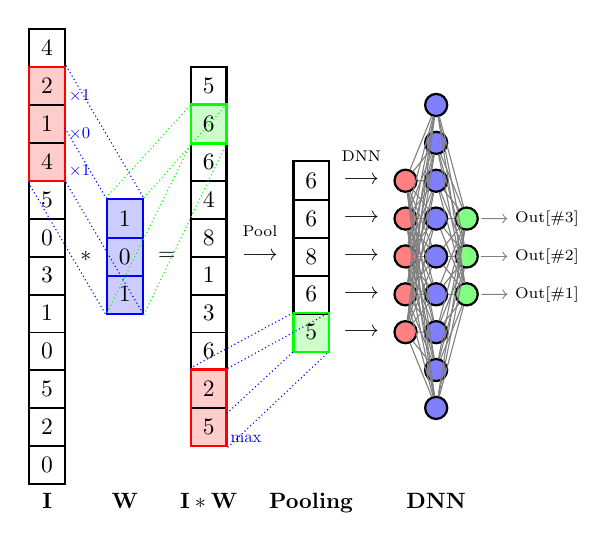
\begin{tikzpicture}[draw=black!50, mmat/.style={matrix of math nodes,column sep=-\pgflinewidth/2,
       row sep=-\pgflinewidth/2,cells={nodes={draw,inner sep=5pt,ultra thin, scale=0.85}},draw=#1,thick,inner sep=0pt},
       mmat/.default=black,
       node distance=0.3em,
       transform shape,scale=0.8]
    
    
    \tikzstyle{every pin edge}=[<-,shorten <=1pt]
    \tikzstyle{neuron}=[circle,fill=black!25,minimum size=10pt,inner sep=0pt]
    \tikzstyle{input neuron}=[neuron, fill=red!50];
    \tikzstyle{output neuron}=[neuron, fill=green!50];
    \tikzstyle{hidden neuron}=[neuron, fill=blue!50];
    \tikzstyle{annot} = [text width=4em, text centered]
    
    
    
     \matrix[mmat](mat1){
            {\scriptsize 4} \\ 
            {\scriptsize 2} \\ 
            {\scriptsize 1} \\ 
            {\scriptsize 4} \\ 
            {\scriptsize 5} \\ 
            {\scriptsize 0} \\ 
            {\scriptsize 3} \\
            {\scriptsize 1} \\
            {\scriptsize 0} \\
            {\scriptsize 5} \\
            {\scriptsize 2} \\
            {\scriptsize 0} \\
            };
     \def\myarray{{1},{0},{1}}       
    \foreach \Y in {0,1,2}
        {\foreach \X in {0}
            {\pgfmathsetmacro{\myentry}{{\myarray}[\Y][\X]}
            \path (mat1-\the\numexpr\Y+2\relax-1.south east)
            node[anchor=south west,blue,scale=0.75,inner sep=2.2pt]{$\times\myentry$};
    }}         
    \node[fit=(mat1-2-1)(mat1-4-1),inner sep=0pt,draw,red,thick,name path=fit](f1){};      
    \node[right=of mat1] (mul) {$*$};      
    \matrix[mmat=blue,fill=blue!20,right=of mul,name path=mat2](mat2){    
        1 \\ 
        0 \\ 
        1 \\ };
    \node[right=of mat2] (eq) {$=$};       
    \matrix[mmat,right=of eq](mat3){
        5 \\
        |[alias=4]|6 \\ 
        6 \\ 
        4 \\ 
        8 \\ 
        1 \\
        3 \\
        6 \\
        2 \\
        5 \\
    };
    \node[fit=(mat3-2-1)(mat3-2-1),inner sep=0pt,draw,green,thick,name path=not_to_consider](ntc){};
    \node[fit=(mat3-9-1)(mat3-10-1),inner sep=0pt,draw,red,thick,name path=fit2](f2){};
    \node[right=of mat3, label={\scriptsize Pool}] (pool) {$\longrightarrow$};
    \matrix[mmat,right=of pool,name path=mmat3](mat4){    
        6 \\ 
        6 \\ 
        8 \\
        6 \\
        |[alias=2]|5 \\
    };
    \node[fit=(mat4-5-1)(mat4-5-1),inner sep=0pt,draw,green,thick,name path=fit3](f3){};
    \node[right=of mat4-1-1, label={\scriptsize DNN}] (DNN1) {$\longrightarrow$};
    \node[right=of mat4-2-1] (DNN2) {$\longrightarrow$};
    \node[right=of mat4-3-1] (DNN3) {$\longrightarrow$};
    \node[right=of mat4-4-1] (DNN4) {$\longrightarrow$};
    \node[right=of mat4-5-1] (DNN5) {$\longrightarrow$};
    
    
    
    
    
    \node[input neuron, draw=black!100, thick, right=of DNN1] (I-1){}; 
    \node[input neuron, draw=black!100, thick, right=of DNN2] (I-2){}; 
    \node[input neuron, draw=black!100, thick, right=of DNN3] (I-3){}; 
    \node[input neuron, draw=black!100, thick, right=of DNN4] (I-4){}; 
    \node[input neuron, draw=black!100, thick, right=of DNN5] (I-5){};
    
    \node[hidden neuron, draw=black!100, thick, right=\layersep of I-1] (H-3){};
    \node[hidden neuron, draw=black!100, thick, right=\layersep of I-2] (H-4){};
    \node[hidden neuron, draw=black!100, thick, right=\layersep of I-3] (H-5){};
    \node[hidden neuron, draw=black!100, thick, right=\layersep of I-4] (H-6){};
    \node[hidden neuron, draw=black!100, thick, right=\layersep of I-5] (H-7){};
    \node[hidden neuron, draw=black!100, thick] (H-2) at ($ (H-4) !2.0! (H-3) $) {};%above=5pt of H-3] (H-2){};
    \node[hidden neuron, draw=black!100, thick] (H-1) at ($ (H-3) !2.0! (H-2) $) {};%above=5pt of H-2] (H-1){};
    \node[hidden neuron, draw=black!100, thick] (H-8) at ($ (H-6) !2.0! (H-7) $) {};%below=5pt of H-7] (H-8){};
    \node[hidden neuron, draw=black!100, thick] (H-9) at ($ (H-7) !2.0! (H-8) $) {};%below=5pt of H-8] (H-9){};
    
    \node[output neuron, draw=black!100, thick, pin={[pin edge={->}]right:{\scriptsize Out{[}\#2{]}}}, right=\layersep of H-5] (O-2){};
    \node[output neuron, draw=black!100, thick, pin={[pin edge={->}]right:{\scriptsize Out{[}\#1{]}}}, right=\layersep of H-6] (O-1){};
    \node[output neuron, draw=black!100, thick, pin={[pin edge={->}]right:{\scriptsize Out{[}\#3{]}}}, right=\layersep of H-4] (O-3){};
    
    \foreach \source in {1,...,5}
        \foreach \dest in {1,...,9}
            \path (I-\source) edge (H-\dest);
    
    \foreach \source in {1,...,9}
        \path (H-\source) edge (O-1);
    \foreach \source in {1,...,9}
        \path (H-\source) edge (O-2);
    \foreach \source in {1,...,9}
        \path (H-\source) edge (O-3);
    
    
    
    
    
    
     \foreach \Anchor in {south west,north west,south east,north east}
     {\path[name path=test] (f1.\Anchor) -- (mat2.\Anchor);
     \draw[blue,densely dotted,name intersections={of=test and fit,total=\t}]
     \ifnum\t>0 (intersection-\t) -- (mat2.\Anchor) \else
      (f1.\Anchor) -- (mat2.\Anchor)\fi;
      
     \path[name path=test2]  (4.\Anchor) -- (mat2.\Anchor);  
     \draw[green,densely dotted,name intersections={of=test2 and mat2,total=\tt}] 
     \ifnum\tt>0 (intersection-1) -- (4.\Anchor) \else
        (mat2.\Anchor) --  (4.\Anchor)\fi;
    
     \path[name path=test3] (f2.\Anchor) -- (mat4.\Anchor);
     \draw[blue,densely dotted,name intersections={of=test3 and fit2,total=\t}]
     \ifnum\t>0 (intersection-\t) -- (2.\Anchor) \else
      (f2.\Anchor) -- (2.\Anchor)\fi;
        }
        
     \path (mat3-10-1.south east) node[anchor=south west,blue,scale=0.75,inner sep=2.2pt]{max};
     \path (mat1.south) node[below] {$\mathbf{I}$}
      (mat2|-mat1.south) node[below] {$\mathbf{W}$}
      (mat3|-mat1.south) node[below] {$\mathbf{I}*\mathbf{W}$}
      (mat4|-mat1.south) node[below] {\textbf{Pooling}}
      (H-5|-mat1.south) node[below] {\textbf{DNN}};
      
    \begin{scope}[on background layer]
        \fill[red!20] (f1.north west) rectangle (f1.south east);
    \end{scope}
    \begin{scope}[on background layer]
        \fill[red!20] (f2.north west) rectangle (f2.south east);
    \end{scope}
    \begin{scope}[on background layer]
        \fill[green!20] (ntc.north west) rectangle (ntc.south east);
    \end{scope}
    \begin{scope}[on background layer]
        \fill[green!20] (2.north west) rectangle (2.south east);
    \end{scope}
    %dobbiamo giusto sistemare un po' la forma e i plot (da mettere tutti in pdf per tenere la grafica vettoriale e sistemare le dimensioni perché forse sono un po' piccoli, ma se vuoi posso farlo io)
    %nah vabbe ho già tutti i codici e so dove cercarli quindi faccio io in scialla (magari domani che oggi sto a pezzi)
    % ahahahahaah sai dopo due mesi che non vedo mia morosa 
    % diciamo che mi serve un po di riposo... ahhaa esatto
    % ok buona cena... mi sa domani perchè tra un po dormiro (io ceno alle 19 ) ahahahah 
    % scialla domani mattina mi metto e vado giu di grafici cosi li abbimamo tutti belli
    % a domani... buona cena rocco
    % * meritato riposo
    % ok, a domani allora 
    % Dai, io vado a cenare, ci sentiamo poi dopo o domani. Ma io sono terrone ahahhahah
    %ma cosa hai combinato per stare così a pezzi ahahhahahahh dio can ahahahahah
    %si infatti.. è venuto been anche come struttura secondo me
    %sempre che latex non si svegli improvvisamente girato
    %non sono molto in me però mi piace
\end{tikzpicture}%%%%%%%%%%%%%%%%%%%%%%%%%%%%%%%%%%%%%%%%%%%%%%%%%
%\end{minipage}
%\begin{minipage}{0.2\columnwidth}
%
%    \begin{tikzpicture}[shorten >=1pt,->,draw=black!50, node distance=\layersep, scale=0.5, transform shape]
%        \tikzstyle{every pin edge}=[<-,shorten <=1pt]
%        \tikzstyle{neuron}=[circle,fill=black!25,minimum size=10pt,inner sep=0pt]
%        \tikzstyle{input neuron}=[neuron, fill=green!50];
%        \tikzstyle{output neuron}=[neuron, fill=red!50];
%        \tikzstyle{hidden neuron}=[neuron, fill=blue!50];
%        \tikzstyle{annot} = [text width=4em, text centered]
%    
%        % Draw the input layer nodes
%        \foreach \name / \y in {1,...,5}
%        % This is the same as writing \foreach \name / \y in {1/1,2/2,3/3,4/4}
%            %\node[input neuron, draw=black!100, thick, pin=left:{\scriptsize In{[}\#\y{]}}] (I-\name) at %(-\layersep,-1.5-1*\y) {};
%            \node[input neuron, draw=black!100, thick] (I-\name) at (-\layersep,-1.5-1*\y) {};
%    
%        % Draw the hidden layer nodes
%        \foreach \name / \y in {1,...,9}
%            \path[yshift=0.5cm]
%                node[hidden neuron,draw=black!100,thick] (H-\name) at (\layersep,-\y cm) {};
%    
%        % Draw the output layer node
%        \node[output neuron,draw=black!100,thick,pin={[pin edge={->}]right:{\scriptsize Out{[}\#1{]}}}, right %of=H-4] (O1) {};
%        \node[output neuron,draw=black!100,thick,pin={[pin edge={->}]right:{\scriptsize Out{[}\#2{]}}}, right %of=H-5] (O2) {};
%        \node[output neuron,draw=black!100,thick,pin={[pin edge={->}]right:{\scriptsize Out{[}\#3{]}}}, right %of=H-6] (O3) {};
%    
%        % Connect every node in the input layer with every node in the
%        % hidden layer.
%        \foreach \source in {1,...,5}
%            \foreach \dest in {1,...,9}
%                \path (I-\source) edge (H-\dest);
%    
%        % Connect every node in the hidden layer with the output layer
%        \foreach \source in {1,...,9}
%            \path (H-\source) edge (O1);
%        \foreach \source in {1,...,9}
%            \path (H-\source) edge (O2);
%        \foreach \source in {1,...,9}
%            \path (H-\source) edge (O3);
%    
%        % Annotate the layers
%        %\node[annot,above of=H-1, node distance=1.0cm] (hl) {Hidden layer};
%        %\node[annot,left of=hl] {Input layer};
%        %\node[annot,right of=hl] {Output layer};
%    \end{tikzpicture}
%\end{minipage}
    \caption{1D basic CNN convolution and pooling operations. The flattened pooling output is then connected to a basic DNN.}
    \label{fig:I_CNN_1D}
\end{figure}

%\textcolor{red}{In machine learning applications, the input is usually a multidimensional array of data, and the kernel (in blue in \figref{fig:I_CNN_1D}) is usually a multidimensional array of parameters to train through the learning algorithm. In a certain layer, we can also have $n\ge1$ kernels applied to $m\ge1$ input levels, giving $n \cdot m$ output levels. The dimensionality of these results is reduced by pooling layers, which apply an operation like average or max/min in blocks.}



\section{Methods}
\paragraph{\bf Data generation:}
First of all, we introduce some notations for the sake of simplicity. We denote with
\begin{align}
    \tilde{x}_j &=  \{ \tilde{x}(t_{1}), \dots, \tilde{x}(t_{L}) \}   \label{eq:x_tilde}  \\
    \hat{x}_j   &=  \{ \hat{x}(t_{L-i+1}), \dots, \hat{x}(t_{L-i+Z}) \}   \label{eq:x_hat}
\end{align}
respectively the $j^{\text{th}}$ input time-series without the bump and the bump itself. The parameters $L$ and $Z$ are respectively the time-series and bump lengths, fixed to 60 and 12, and $i$ ranges from $Z$ to $L$.

$\tilde{x}_j(t)$ signals are generated by sampling the amplitude difference $\mathrm{d}x$ between $\tilde{x}_j(t_{i})$ and $\tilde{x}_j(t_{i+1})$, from an exponential probability distribution:
\begin{equation}
    \mathbb{P}(\mathrm{d}x) \sim \operatorname{exp}\left(-\frac{|\mathrm{d}x - b|}{\Delta x}\right)
    \label{eq:M_P}
\end{equation}
where $b$ is a parameter called bias and $\Delta x$ is the step typical size of the jump process. In our case, they are fixed respectively to 5 and 50. By applying the inverse transform of Eq. \ref{eq:M_P}, we get the sampling rule:
\begin{equation}
    \mathrm{d}x = \floor*{\log(p) \Delta x} \cdot 2 \operatorname{sign}(q - 0.5) + b
    \label{eq:M_DX}
\end{equation}
where $p$ is a random number sampled from a uniform distribution in $[0,1]$,  $q$ is chosen in $\{0,1\}$ with equal probability assigned to each element of the set.

$\hat{x}_j(t)$ signals are sine bumps generated through:
\begin{equation}
    %int(a * math.sin((math.pi*i)/z))
    \hat{x}_j(t_{i+k}) = \floor*{A \cdot \sin\left( \frac{\pi \cdot k}{Z} \right)}
    \label{eq:M_DX}
\end{equation}
where $A$ is the amplitude of the signal, initially fixed to 500. As we can deduce from Eq. \ref{eq:x_hat}, they are added randomly inside the time-series.

Hence, we have three possibilities for the input signals, properly labeled by a target variable $y$:
\begin{equation}
    x_j = 
    \begin{cases}
        \tilde{x}_j + 0 \cdot \hat{x}_j     &\qquad   y_j=0     \\
        \tilde{x}_j + 1 \cdot \hat{x}_j     &\qquad   y_j=1     \\
        \tilde{x}_j - 1 \cdot \hat{x}_j     &\qquad   y_j=2     \\
    \end{cases}
    \label{eq:M_X}
\end{equation}
These data are normalized before feeding them to the CNN. This is done by subtracting the mean of the time-series and by dividing by the standard deviation.

\begin{figure*}[!tb]
    \begin{minipage}{0.66\columnwidth}
        {\footnotesize
        \begin{tabular}{ccc}
            \toprule
            Layer type & Output shape & Parameters \\
            \colrule
            Conv1D & (50,5) & 60 \\
            Av. Pool. & (16, 5) &0 \\
            %\hline
            Conv1D & (10,5) & 180 \\
            %\hline
            Av. Pool. & (5, 5) & 0 \\
            %\hline
            Conv1D & (1,5) & 130 \\
            %\hline
            Flatten & (5) &0 \\
            %\hline
            Dense & (10) & 60 \\
            %\hline
            Dense & (10) & 110 \\
            %\hline
            Dropout$(0.2)$ & (10) & 0 \\
            %\hline
            Dense & (3) & 33 \\
            \botrule
        \end{tabular}}
    \end{minipage}
    \hfill
    \begin{minipage}{0.66\columnwidth}
        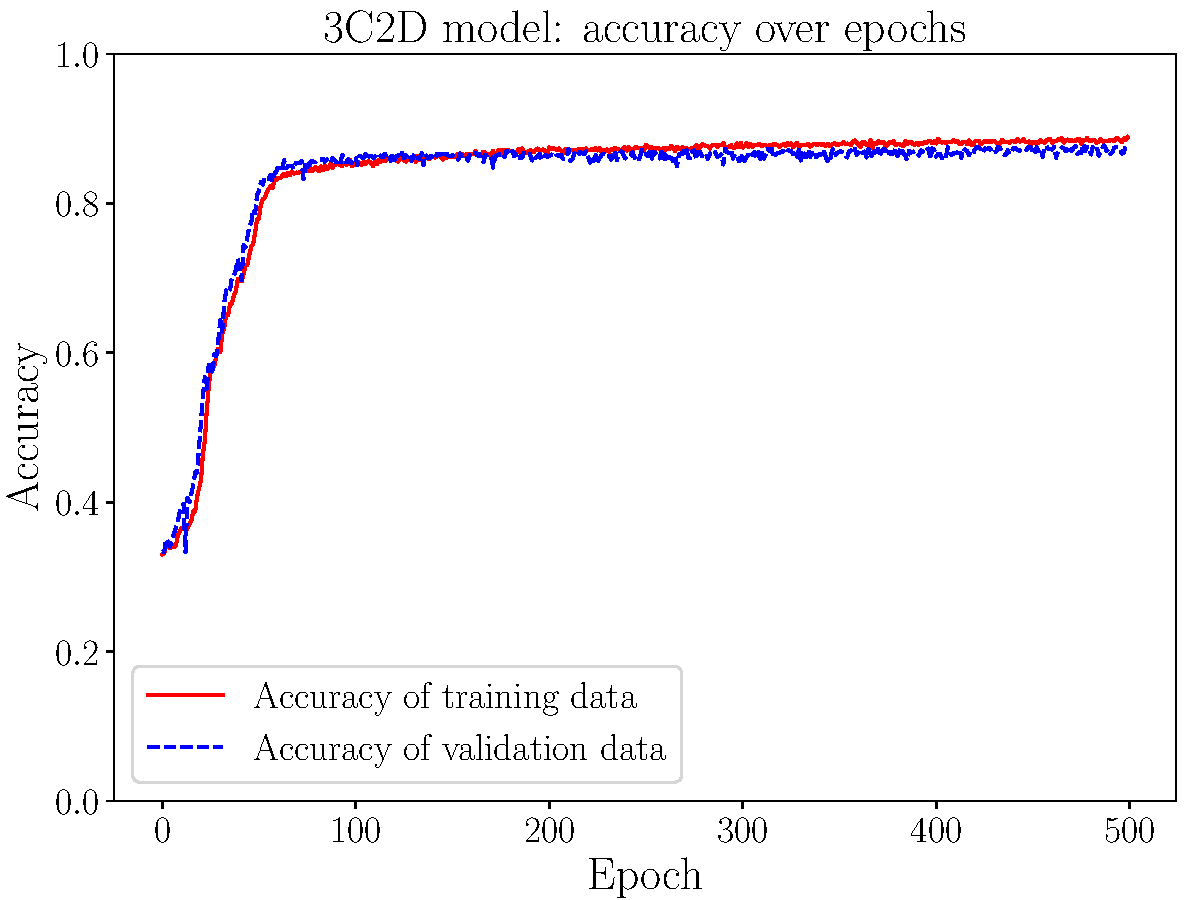
\includegraphics[width=\textwidth]{Images/Results/3C2D_accs.pdf}
    \end{minipage}
    \hfill
    \begin{minipage}{0.66\columnwidth}
        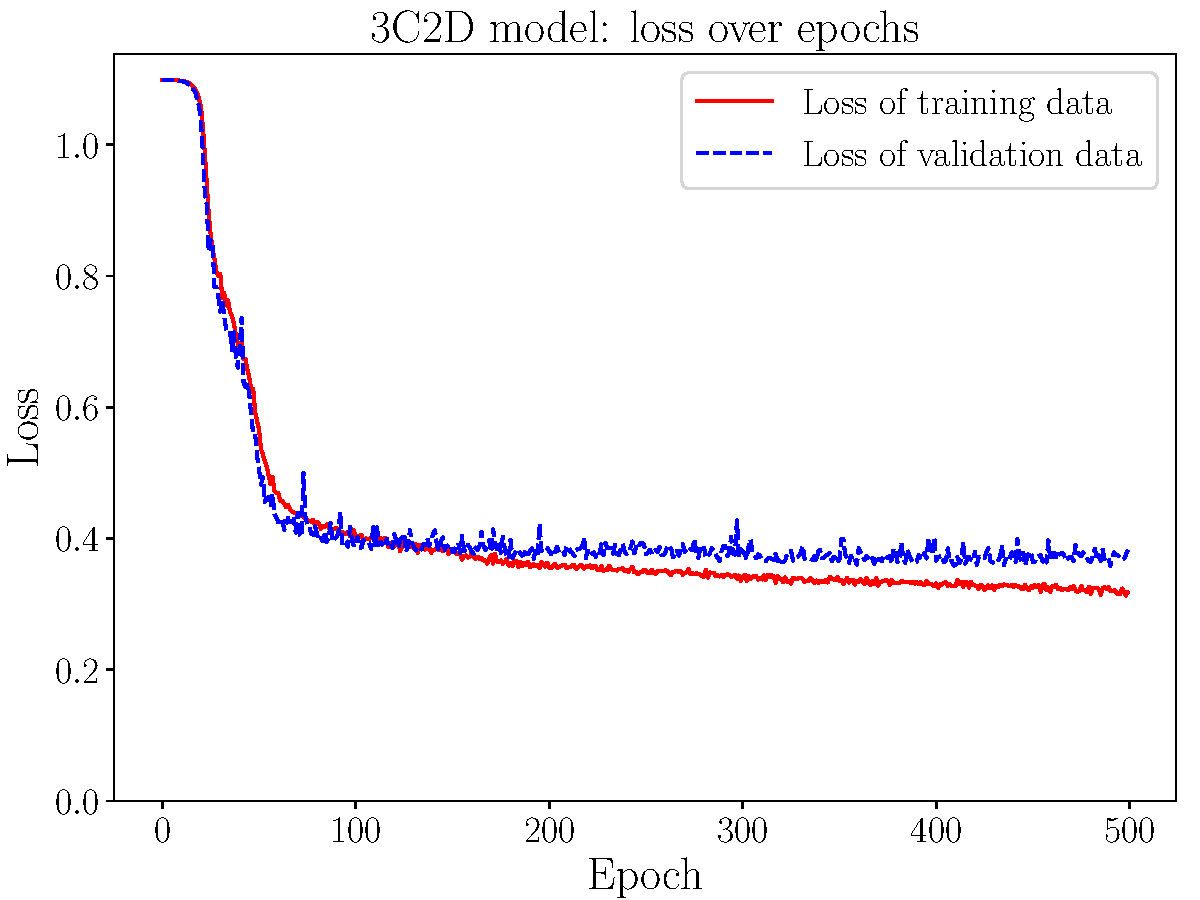
\includegraphics[width=\textwidth]{Images/Results/3C2D_losses.pdf}
    \end{minipage}
    
    \caption{Detailed architecture of the best performing model (3C2D) on the left. Results for this architecture on the right.}
    \label{fig:best_accu}
\end{figure*}



\paragraph{\bf CNN implementation:}
The networks are built through the powerful python libraries of TensorFlow and Keras, which allow to implement even complex CNNs and DNNs in few lines of code. One of our aims is to find the best performing architecture; to do this we have divided the first part of the work into two steps:
\begin{itemize}
    \item in the first one we compare various CNN architectures, created from a reference model (``2C1D'') by varying the number of Convolutional or Dense layers. A constraint on the number of parameters is set in order to avoid too complex models. After training them with the same conditions, we select the one with the highest maximum accuracy;
    \item in the second step, we analyze how the best architecture can be tuned by optimizing the hyperparameters through grid searches with a $3$-fold cross validation method. More deeply, we focus on the tuning of the optimizer and the regularizer.
    %\item In the last part we analyzed which was the ``threshold'' of signal to noise ratio for our model to be still effective.
\end{itemize}
%By constraining the number of trainable parameters to $600$, we were able to build $5$ different models by starting from a reference one with two Conv1D and one Dense layers. In particular, we observed how the accuracy and loss over training epochs for the reference model react by augmenting the number of dense or convolutional layers.

%Once the best model is chosen, we tried to improve its accuracy by tuning the parameters, activation function of the Dense layers, the solver and introducing a regularization in the kernel.

%This operation was done performing a grid search with the various parameters and functions, starting from coarser grids and slowly changing to finer ones to select the best options. In addiction we used also a $3$-fold cross-validation in order to obtain a better estimation even with a smaller dataset, in order to reduce the computational weight.

After these steps we are able to define the best model for data classification. So, in the last part of our work we try to train the model using datasets where signal-to-noise ratio is reduced progressively. This operation translates into generating datasets with a lower signal amplitude $A$, allowing us to estimate a threshold under which the model is not capable of effectively classifying the data.

%allowing us to find out which is the threshold for the model to be still capable of correctly classify the data.
Moreover, we try to maximize the stability and capability of the model of making correct predictions. For this last run we generate a dataset with more samples in comparison to the previous ones, but with a signal amplitude randomly chosen between the starting value and the previously defined threshold. After training and test phases, we exploit the confusion matrix of the predictions to better understand the behaviour of the network for each data category.





 

\section{Results}
The different architectures are presented in \tabref{tab:R_arch} alongside with their score, namely the maximum accuracy on the validation set obtained during training. As we can see. the most important factor affecting the results seems to be the number of layers, rather than the number of parameters. In fact, we can observe that the best architectures are the ones with more layers despite having less parameters respect to the others. In  \figref{fig:best_accu}, the plots of accuracy and loss function over the training epochs, are showed for the best architecture, alongside with a detailed description of the architecture of that model. 








\begin{table}
    \centering
    \begin{tabular}{ccc}
        \toprule
        \textbf{Model} & \textbf{Parameters} & \textbf{Score}   \\
        \colrule
        1C1D & $587$ & $88.4\%$ \\
        2C1D & $579$ & $88.8\%$ \\ 
        2C2D & $593$ & $89.1\%$ \\ 
        3C1D & $598$ & $88.7\%$ \\ 
        \textcolor{red}{\bf 3C2D}  & 
        \textcolor{blue}{$\mathbf{573}$} & 
        \textcolor{blue}{$\mathbf{89.3\%}$} \\
        \botrule
    \end{tabular}
    \caption{Training results on different CNN architectures, training set of $8000$ events with signal amplitude of $500$, training performed with a batch size of $250$ for $500$ epochs. The name of the models describes their structure: ``C'' indicates a Convolutional layer, ``D'' a hidden Dense one and the number beside how many per type are present.}
    \label{tab:R_arch}
\end{table}

%\vspace{-5pt}




%\onecolumngrid
%\begin{widetext}
%\begin{minipage}{0.33\textwidth}
%\small
%\begin{tabular}{lcc}
%\toprule
%Layer type & Output shape & Parameters \\
%%\hdashline
%%\hdashline
%Conv. 1D & (50,5) & 60 \\
%\hline
%Av. Pooling & (16, 5) &0 \\
%\hline
%Conv. 1D & (10,5) & 180 \\
%\hline
%Av. Pooling & (5, 5) & 0 \\
%\hline
%Conv. 1D & (1,5) & 130 \\
%\hline
%Flatten & (5) &0 \\
%\hline
%Dense & (10) & 60 \\
%\hline
%Dense & (10) & 110 \\
%\hline
%Dropout $20\%$ & (10) & 0 \\
%\hline
%Dense & (3) & 33 \\
%\botrule
%\end{tabular}
%\end{minipage}
%\begin{minipage}{0.33\textwidth}
%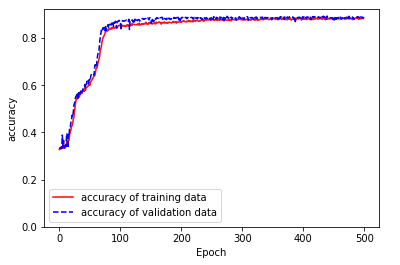
\includegraphics[width=\textwidth]{Images/acc3c2d.png}
%\end{minipage}
%\begin{minipage}{0.33\textwidth}
%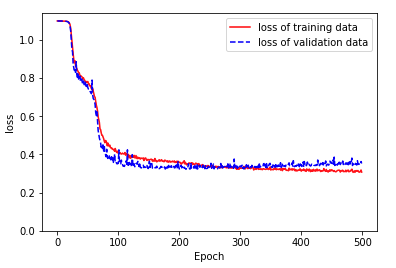
\includegraphics[width=\textwidth]{Images/loss3c2d.png}
%\end{minipage}
%\end{widetext}
%\twocolumngrid
%
%\begin{comment}
%\begin{figure*}[!tb]
%    \centering
%    \includegraphics[width=0.55\textwidth]{Images/3c2d.png}
%    \hskip 1mm
%    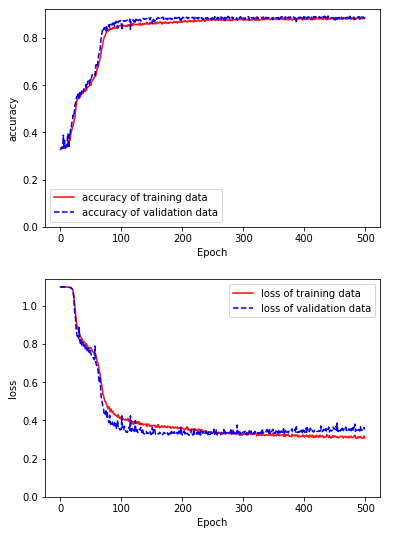
\includegraphics[width=0.4\textwidth]{Images/3c2daccloss.png}
%
%    \caption{Description of the panels: The images refer to the best architecture for the task, in particular: a) represent the architecture of the model, b) is the plot of the accuracy on the training and validation set during the train and c) is the plot of the loss function}
%    \label{fig:best_accu}
%\end{figure*}
%\end{comment}
\begin{figure*}[!t]
    \centering 
    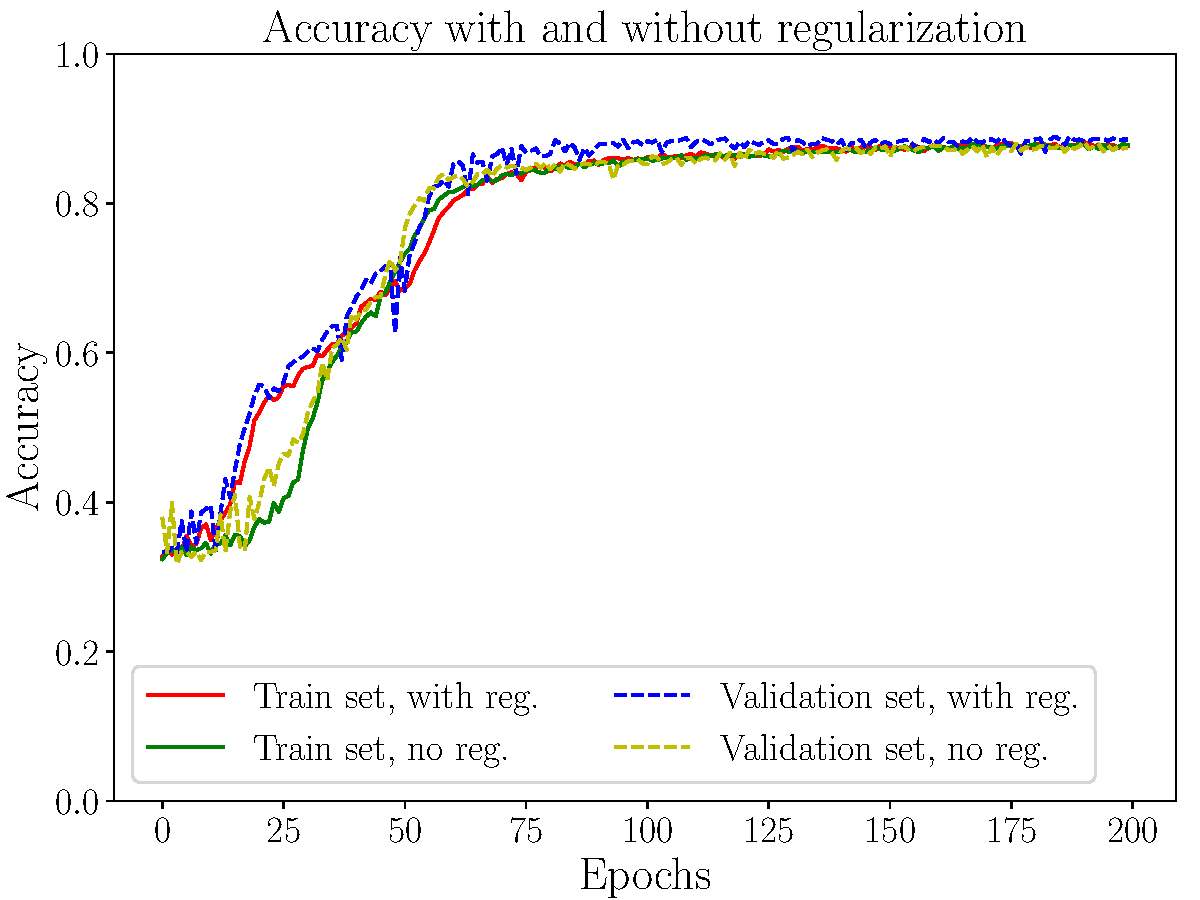
\includegraphics[width=0.32\textwidth]{Images/Results/Acc_reg.pdf}
    \hskip 1mm
    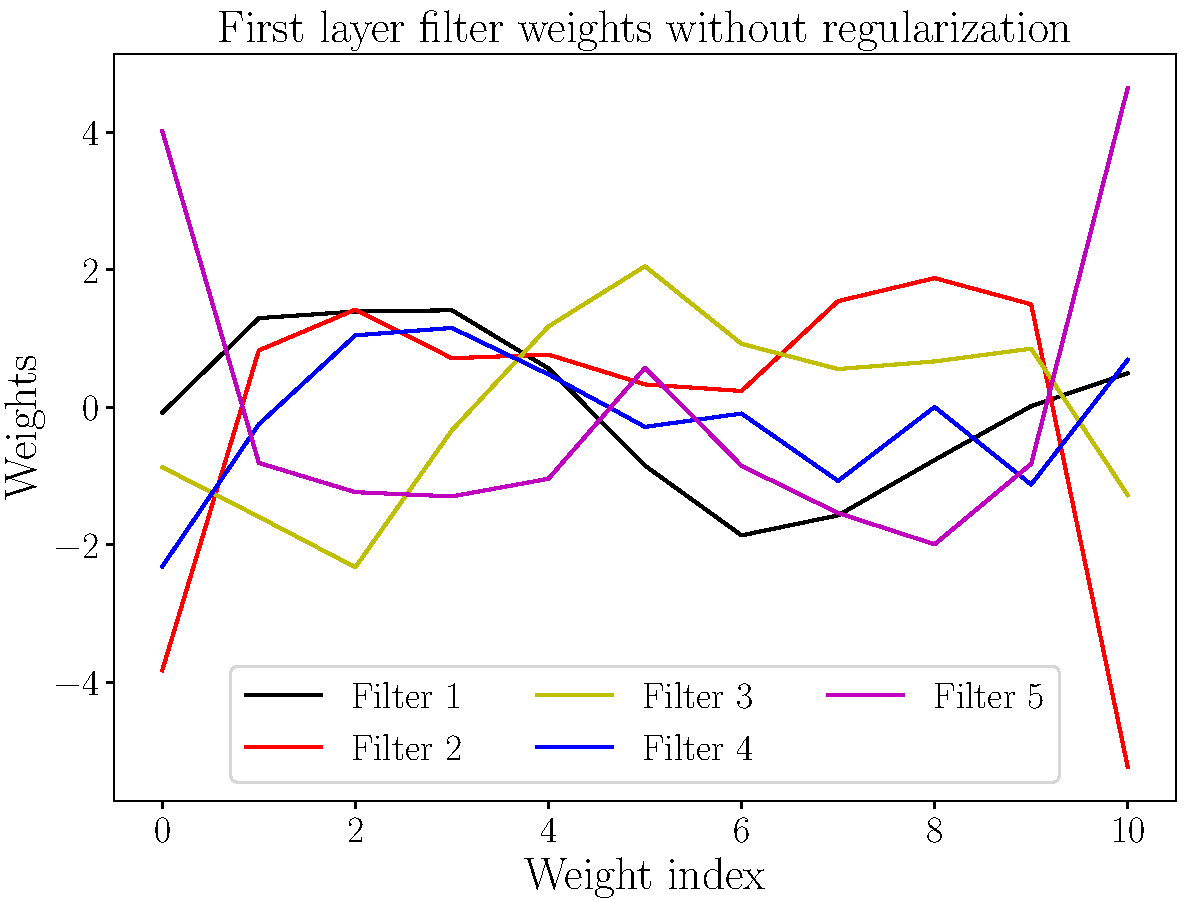
\includegraphics[width=0.32\textwidth]{Images/Results/Weights_noReg.pdf}
    \hskip 1mm
    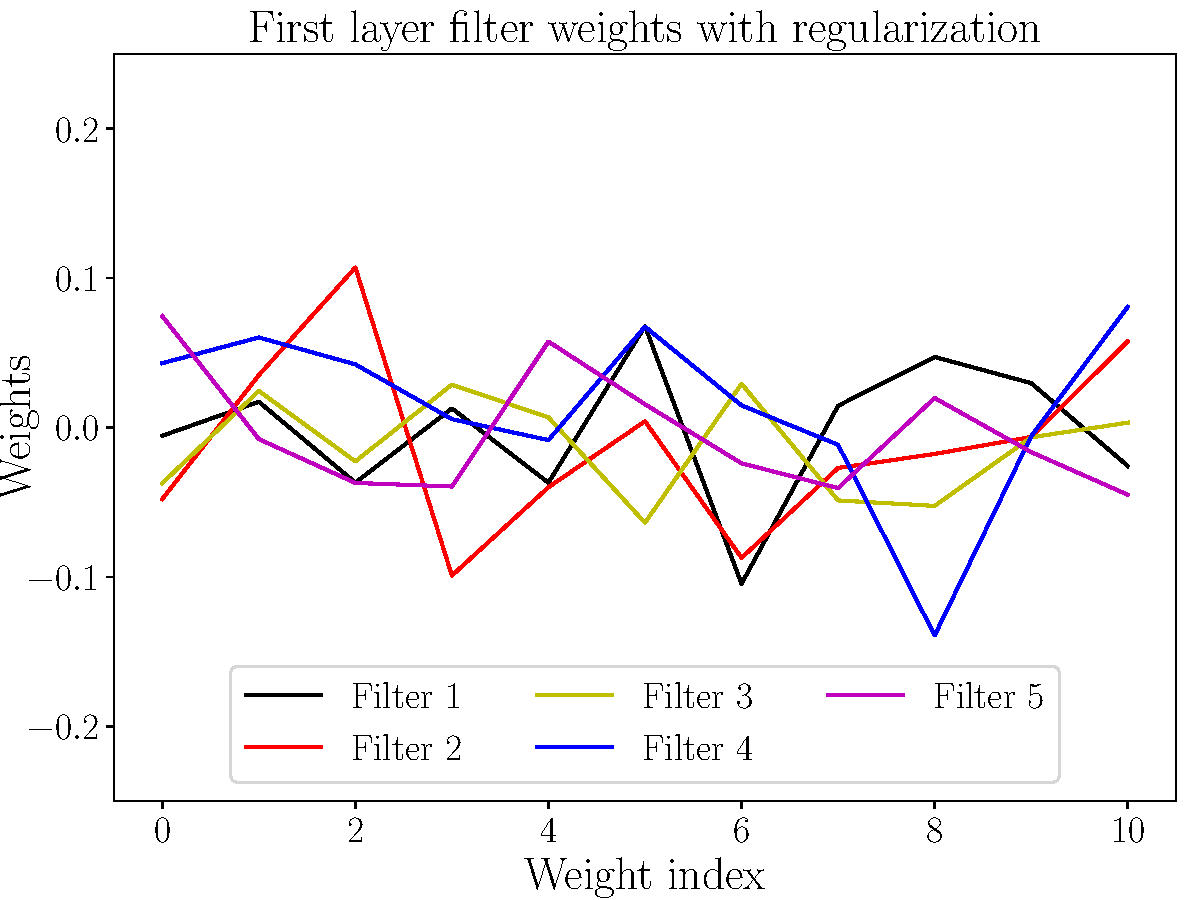
\includegraphics[width=0.32\textwidth]{Images/Results/Weights_reg.pdf}

    \caption{Left: accuracy of the model during training with and without regularization. Center and right: weights of the filters of the first layer with and without regularization.}
    \label{fig:weights}
\end{figure*}
\begin{figure*}[!t]
    \centering 
    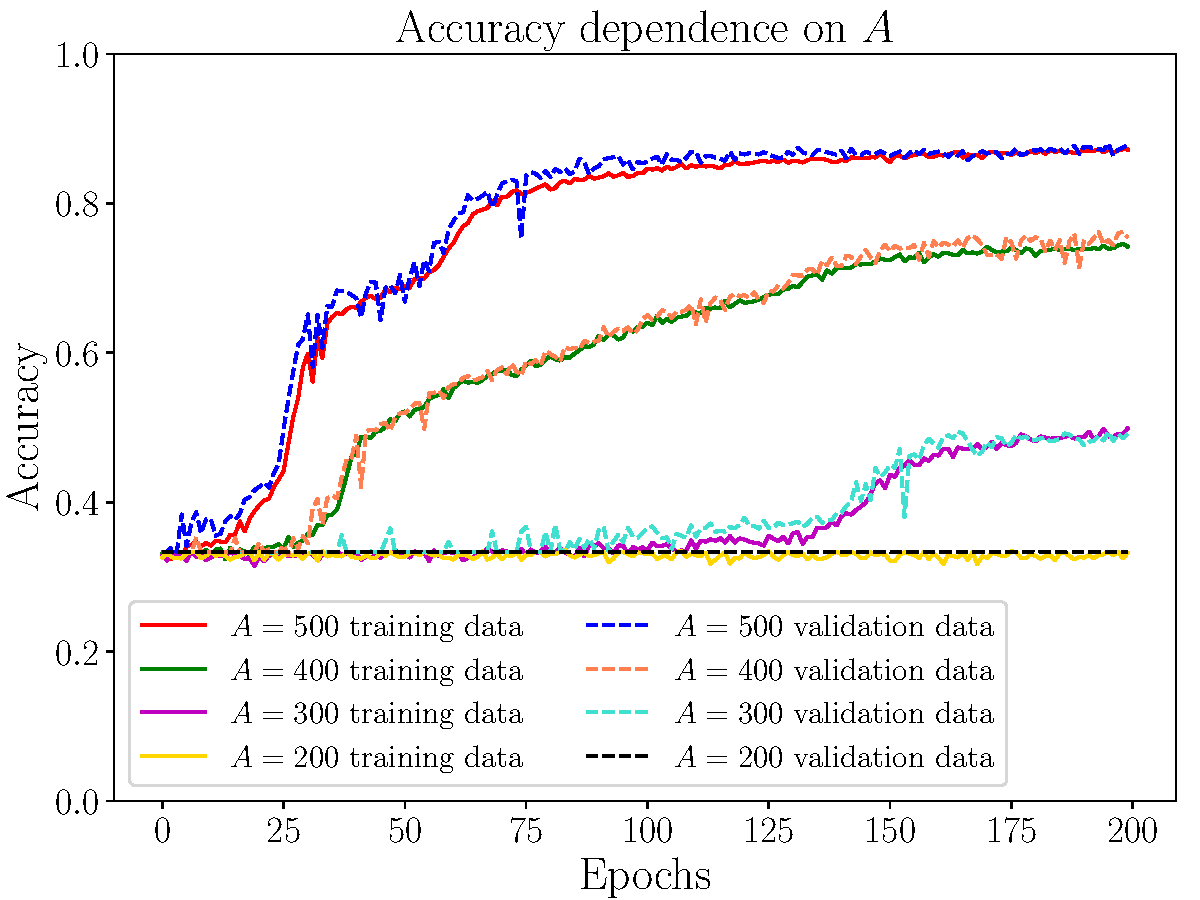
\includegraphics[width=0.32\textwidth]{Images/Results/A_acc_SNR.pdf}
    \hskip 1mm
    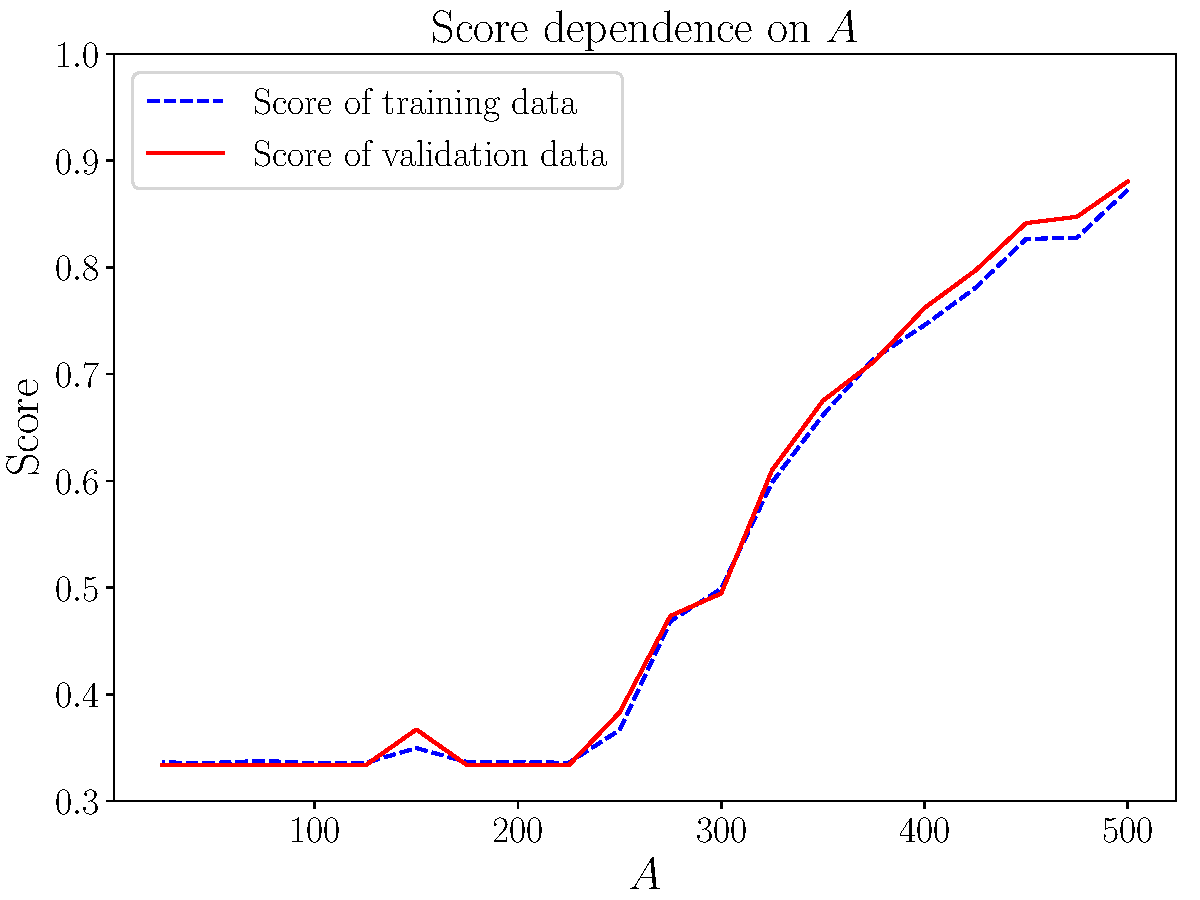
\includegraphics[width=0.32\textwidth]{Images/Results/SNR_A_acc_over_A.pdf}
    \hskip 1mm
    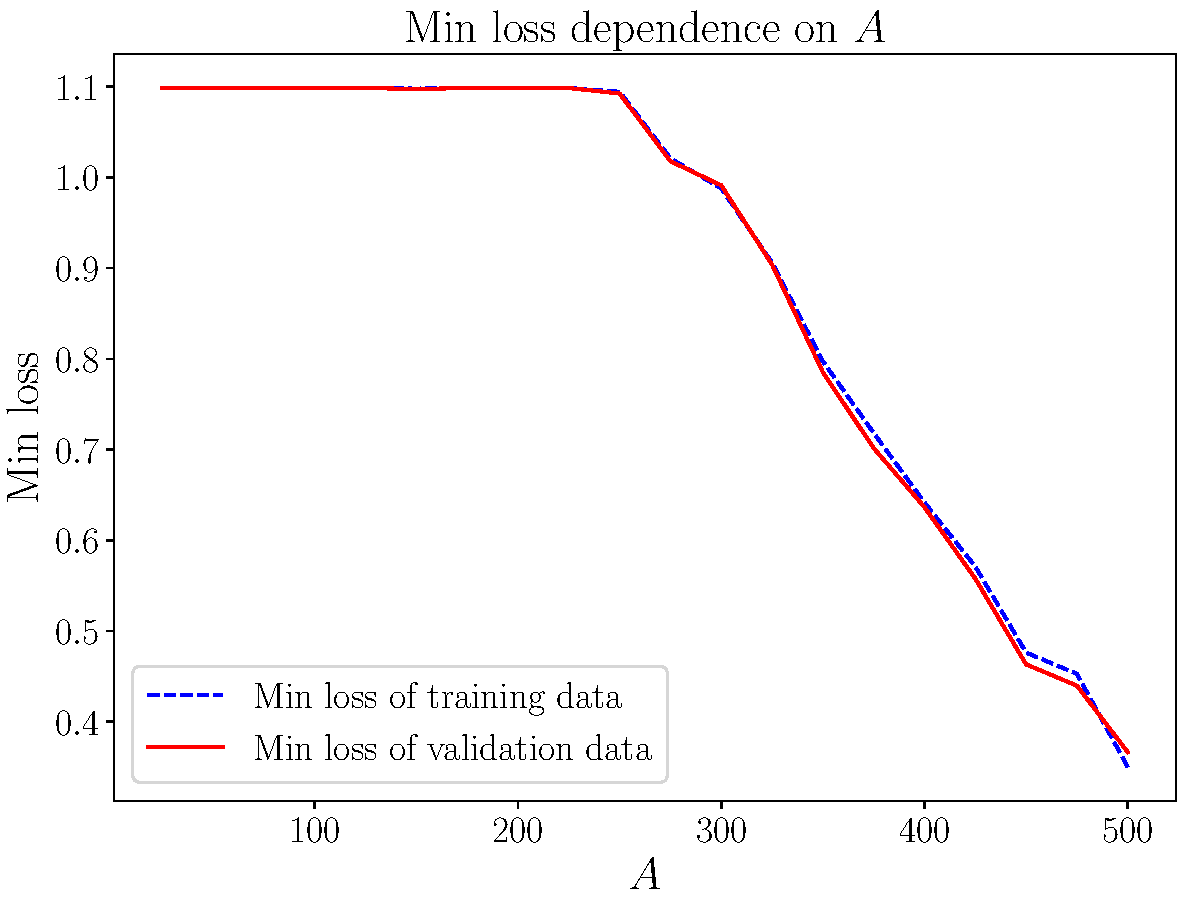
\includegraphics[width=0.32\textwidth]{Images/Results/SNR_A_loss_over_A.pdf}

    \caption{Left: accuracy of the model during training for datasets with different signal amplitudes. Center and right: score and loss dependence on $A$.}
    \label{fig:ratio}
\end{figure*}

\begin{comment}
Per giocare con il grafico il codice è (senza dover rigirare tutto perchè ci vuol un ora
As=[ 500,475, 450, 425, 400, 375, 350,325,  300, 275, 250, 225, 200, 175, 150, 125, 100, 75,50, 25, 10]
y_acc=[0.896, 0.887, 0.885, 0.882, 0.884, 0.845, 0.851, 0.832, 0.789, 0.775 ,0.764, 0.725,
 0.591 ,0.531, 0.478 ,0.425, 0.404,0.4 ,  0.348 ,0.383 ,0.368]
y_loss=[0.376 ,0.384 ,0.363 ,0.357 ,0.423 ,0.47 , 0.429 ,0.505 ,0.583, 0.645, 0.722 ,0.813,
 0.952, 0.999 ,1.048, 1.082 ,1.09 , 1.095 ,1.099 ,1.097, 1.098]
 
plt.rc('font', size=16)          # controls default text sizes
plt.rc('axes', titlesize=18)     # fontsize of the axes title
plt.rc('axes', labelsize=18)    # fontsize of the x and y labels
plt.rc('xtick', labelsize=14)    # fontsize of the tick labels
plt.rc('ytick', labelsize=14)    # fontsize of the tick labels
plt.rc('legend', fontsize=14)    # legend fontsize
plt.rc('figure', titlesize=18)  # fontsize of the figure title


plt.plot(As, y_acc, 'r', label='Accuracy of test data')
plt.plot(As, y_loss, 'b--', label='Loss of test data')
plt.title("Accuracy dependance on A")
plt.xlabel("Signal-to-noise ratio")
#plt.ylabel("Scores")
plt.legend()
plt.ylim(0)
plt.savefig("avar.png")



\end{comment}







The best model is then tuned by performing several grid searches to find the best configuration.
%In particular, we tune:
%\begin{itemize}
%    \itemsep0em
%    \item the optimizer algorithm;
%    \item the parameters of the optimizer;
%    \item the activation function of each layer;
%    \item the dropout rate.
%\end{itemize}
%
In \tabref{tab:opt} and \tabref{tab:reg} are respectively presented some of the most significant results obtained during this phase, focusing particularly on the optimization algorithms and the regularization functions.
%We find as best configuration the combination of the Nesterov-SGD optimizer with an L$1$ regularization function.
For the sake of simplicity, we report a summary of the parameters of the best setup:
\begin{itemize}
    \itemsep0em
    \item \textbf{Optimizer}: Nesterov-SGD with learning rate $0.02$, momentum $0.9$ and decay $10^{-6}$.
    \item \textbf{Activation functions}: ``relu'' activations for all the layers expect the last one which uses the ``softmax'', since we want every output entry in $[0,1]$.
    \item \textbf{Dropout rate}: $p=0.2$.
    \item \textbf{Regularizer}: L$1$ regularization with $\lambda_\mathrm{L1} = 5\cdot 10^{-6}$.
\end{itemize}
With this configuration our model can reach a test accuracy of $90.6\%$.



\begin{table}[!h]
    \centering
    \begin{tabular}{c|ccccccccc}
        
        \toprule
        \multicolumn{10}{c}{\small\textbf{Optimizer: NAdam}}  \\
        \colrule
        {\small $\eta$}   &   {\scriptsize 0.003} & {\scriptsize 0.005} & {\scriptsize 0.007} & {\scriptsize 0.003} & {\scriptsize \textcolor{blue}{\bf0.005}}  & {\scriptsize 0.007} & {\scriptsize 0.003} & {\scriptsize 0.005}  & {\scriptsize 0.007} \\
        {\small $\beta_1$}&   {\scriptsize 0.85} & {\scriptsize 0.85} & {\scriptsize 0.85} & {\scriptsize 0.875} & {\scriptsize \textcolor{blue}{\bf0.875}}  & {\scriptsize 0.875} & {\scriptsize 0.9} & {\scriptsize 0.9}  & {\scriptsize 0.9} \\
        {\small Score}      &   {\scriptsize 0.868} & {\scriptsize 0.875} & {\scriptsize 0.852} & {\scriptsize 0.693} & {\scriptsize \textcolor{red}{\bf0.878}}  & {\scriptsize 0.874} & {\scriptsize 0.866} & {\scriptsize 0.869}  & {\scriptsize 0.691} \\
        \botrule
        \multicolumn{10}{c}{\small\textbf{Optimizer: RMSprop}}  \\
        \colrule
        {\small $\eta$}&  {\scriptsize 0.01} & {\scriptsize \textcolor{blue}{\bf0.01}}   & {\scriptsize 0.01} & {\scriptsize 0.015} & {\scriptsize 0.015} & {\scriptsize 0.015} & {\scriptsize 0.02} & {\scriptsize 0.02} & {\scriptsize 0.02} \\
        {\small $\rho$}&  {\scriptsize 0.87} & {\scriptsize \textcolor{blue}{\bf0.9}}   & {\scriptsize 0.93} & {\scriptsize 0.87} & {\scriptsize 0.9} & {\scriptsize 0.93} & {\scriptsize 0.87} & {\scriptsize 0.9} & {\scriptsize 0.93} \\
        {\small Score}&  {\scriptsize 0.861} & {\scriptsize \textcolor{red}{\bf0.869}}   & {\scriptsize 0.682} & {\scriptsize 0.672} & {\scriptsize 0.507} & {\scriptsize 0.683} & {\scriptsize 0.513} & {\scriptsize 0.854} & {\scriptsize 0.639} \\
        \botrule
        \multicolumn{10}{c}{\small\textbf{Optimizer: Nesterov-SGD}}  \\
        \colrule
        {\small $\eta$}  & {\scriptsize 0.01} & {\scriptsize 0.01} & {\scriptsize 0.01} & {\scriptsize 0.02} & {\scriptsize 0.02} & {\scriptsize \textcolor{blue}{\bf0.02}} & {\scriptsize 0.03} & {\scriptsize 0.03} & {\scriptsize 0.03} \\
        {\small m}  & {\scriptsize 0.875} & {\scriptsize 0.9} & {\scriptsize 0.925} & {\scriptsize 0.875} & {\scriptsize 0.9} & {\scriptsize \textcolor{blue}{\bf0.925}} & {\scriptsize 0.875} & {\scriptsize 0.9} & {\scriptsize 0.925} \\
        {\small Score}  & {\scriptsize 0.733} & {\scriptsize 0.660} & {\scriptsize 0.675} & {\scriptsize 0.688} & {\scriptsize 0.875} & {\scriptsize \textcolor{darkpastelgreen}{\bf0.882}} & {\scriptsize 0.333} & {\scriptsize 0.10} & {\scriptsize 0.860} \\
        \botrule
    \end{tabular}
    \caption{Cross validated grid search results in the tuning of the regualarization for the model 3C2D.}
    \label{tab:opt} 
    \vspace{2mm}
%\end{table}
%
%\begin{table}[!h]
%    \centering
    \begin{tabular}{c|ccccccccc}
        \toprule
        \multicolumn{10}{c}{\small \bf L1 regularization}  \\
        \colrule
        {\small $\lambda_\mathrm{L1}$} & {\scriptsize 5e-7}      &   {\scriptsize 1e-6}    &   {\scriptsize 3e-6}    &   {\scriptsize\textcolor{blue}{\bf5e-6}}   &   {\scriptsize 8e-6}    &   {\scriptsize 1e-5}    &   {\scriptsize 5e-5}    &   {\scriptsize 1e-4} &   {\scriptsize 5e-4}    \\ 
        {\small Score}  & {\scriptsize 0.692}    &   {\scriptsize 0.871}  &   {\scriptsize 0.868}  &   {\scriptsize \textcolor{darkpastelgreen}{\bf0.881}}  &   {\scriptsize 0.870}  &   {\scriptsize 0.873}  &   {\scriptsize 0.687}  &   {\scriptsize 0.689} &  {\scriptsize 0.506} \\
        \botrule
        \multicolumn{10}{c}{\small \bf L2 regularization}  \\
        \colrule
        {\small $\lambda_\mathrm{L2}$}     &{\scriptsize 5e-6} &
{\scriptsize 1e-5} & {\scriptsize 5e-5} & {\scriptsize 1e-4} & {\scriptsize \textcolor{blue}{\bf3e-4}} & 
{\scriptsize 5e-4} & {\scriptsize 8e-4} & {\scriptsize 1e-3} & {\scriptsize 5e-3}\\
        {\small Score}   &   {\scriptsize 0.775} &{\scriptsize 0.694} & {\scriptsize 0.698} & 
{\scriptsize 0.697} & {\scriptsize \textcolor{red}{\bf0.875}} & {\scriptsize 0.866} & {\scriptsize 0.696} & 
{\scriptsize 0.467} & {\scriptsize 0.638}\\
        \botrule
        \multicolumn{10}{c}{\small \bf L1-L2 regularization}  \\
        \colrule
        {\small $\lambda_\mathrm{L1}$}  &  {\scriptsize 1e-5} & 
{\scriptsize 1e-5} & 
{\scriptsize 1e-5} & 
{\scriptsize 5e-5} & 
{\scriptsize \textcolor{blue}{\bf5e-5}} & 
{\scriptsize 5e-5} & 
{\scriptsize 1e-4} & 
{\scriptsize 1e-4} & 
{\scriptsize 1e-4}\\
        {\small $\lambda_\mathrm{L2}$}  &   {\scriptsize 1e-5} & 
{\scriptsize 5e-4} & 
{\scriptsize 1e-4} & 
{\scriptsize 1e-5} & 
{\scriptsize \textcolor{blue}{\bf5e-4}} & 
{\scriptsize 1e-4} & 
{\scriptsize 1e-5} & 
{\scriptsize 5e-4} & 
{\scriptsize 1e-4}\\
        {\small Score}   & {\scriptsize 0.873} & 
{\scriptsize 0.689} & 
{\scriptsize 0.872} & 
{\scriptsize 0.877} & 
{\scriptsize \textcolor{red}{\bf0.878}} & 
{\scriptsize 0.689} & 
{\scriptsize 0.516} & 
{\scriptsize 0.872} & 
{\scriptsize 0.693} \\
        \botrule
    \end{tabular}
    \caption{Cross validated grid search results in the tuning of the regularization for the model 3C2D.}
    \label{tab:reg}
    
    \vspace{-7mm}
\end{table}

The new best score obtained is a visible enhancement, but there are other improvements hidden in the core of the network. For this reason, we deepen the consequences that the introduction of a regularizer has on the model. As we can see in \figref{fig:weights}, there is a very small improvement in the accuracy. On the other hand, we observe a significant reduction of the magnitude of the filters weights. This evidence translates into a more stable and reliable predictor after the training is completed.


Now that the best architecture is defined, the next step is finding a threshold for the signal amplitude such that the trained model is still reliable in its predictions. Therefore, we generate multiple training and test datasets, with a progressively decreasing signal-to-noise ratio, thus with a decreasing value of $A$. 

We then evaluate the performances of the model on each test set after training on the corresponding training set. Some of the results of this operation are showed in \tabref{tab:ratio} and \figref{fig:ratio}.
%trained the model on different datasets in which the signal to noise ratio has been progressively reduced, teh results of this operation are shown in \tabref{tab:ratio} and \figref{fig:ratio}


\begin{table}[!h]
    \begin{center}
        \begin{tabular}{c|ccccccc}
            \toprule
            %& \multicolumn{8}{c}{\bf Signal-to-noise ratio} \\
            %\colrule
            {\small $\mathbf{A}$}   & {\small\bf 500}       & {\small\bf 450}       & {\small\bf 400}       & {\small\bf 350}       & {\small\bf 300}       & {\small\bf 250}       & {\small\bf 200}       \\
            \colrule
            Score           & {\scriptsize 0.891}   & {\scriptsize 0.841}   & {\scriptsize 0.762}   & {\scriptsize 0.675}   & {\scriptsize 0.495}   & {\scriptsize 0.383}   & {\scriptsize 0.333}   \\
            Min loss        & {\scriptsize 0.366}   & {\scriptsize 0.463}   & {\scriptsize 0.636}   & {\scriptsize  0.785}  & {\scriptsize 0.991}   & {\scriptsize  1.093 } & {\scriptsize 1.099 }  \\
        \botrule
        \end{tabular}
    \end{center}
    \caption{Performances of the best architecture on datasets with different signal amplitude.}
    \label{tab:ratio}
\end{table}

As highlighted by the results, the model is capable of making good predictions down to a signal amplitude of approximately $350$.
In fact, for an amplitude of about $300$ the score is already at $49.5\%$, which does not translate into a completely reliable prediction. When going down to $200$, the score is about $33\%$, which is equivalent to a random guess, since we have $3$ possible equal-probable categories.

The final step is then to experiment if we can further improve the classification power of the best model up to now. The idea is to train it on a bigger dataset of about $10^{6}$ samples with a variable signal amplitude, chosen randomly between $350$ and $500$, to improve the stability and adaptability of the network. We then test the trained model on another test dataset, achieving the best accuracy of our work: $91.5\%$.

%\vspace{-5mm}

\begin{figure}[!ht]
    \centering
    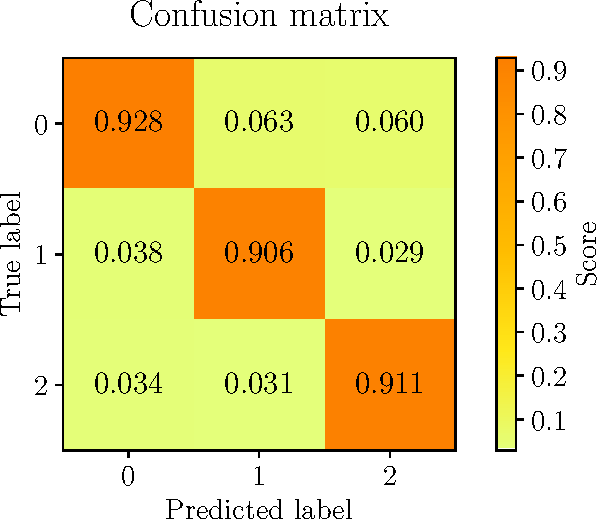
\includegraphics[width=0.64\columnwidth]{Images/Results/3C2D_confusion_matrix.pdf}
    %\vspace{-5mm}
    \caption{Confusion matrix of the best model prediction over a test set with random signal amplitude.}
    \label{fig:confmat}
\end{figure}
%\vspace{-5mm}

A more precise analysis of this result can be extrapolated by the normalized confusion matrix in \figref{fig:confmat}. As we can see, most of the errors are represented by ``false positives'', namely cases where the CNN classifies an input sample as signal despite it being only noise.


%\begin{figure}[!h]
%  \begin{pgfpicture}
%    \pgftext{\pgfimage[width=0.9\columnwidth,height=0.3\textheight]{Images/3C2D_confusion_matrix%.png}}
%  \end{pgfpicture}
%   \caption{Confusion matrix of the best model prediction over a test set}
%\end{figure}




%
%\begin{Huge}
 %   \textcolor{red}{\bf THE ATOMIC RUUN \\ BRUUUUHHHH}
%\end{Huge}





\section{Conclusions}

In this work we highlight the importance of choosing the correct architecture of a CNN for the task. In fact, despite being the one with the lowest amount of parameters, we find the ``$3$C$2$D'' model to be the best choice among the others. 

The study of the stability and the tuning of the network prove to be really important factors in the selection of the architecture. In particular, we show that the most important hyperparameters to tune, in order to achieve a higher score and stability, are the optimizer function, the regularizer and their respective parameters.
%\begin{itemize}
%    \itemsep0em
%    \item the optimezer function and it's parameters;
%    \item the introduction of a regularization function;
%    \item the choice of the activation function.
%\end{itemize}

The other key aspect of this work is the dataset itself. We see that the best model selected is stable and able to make good predictions in a certain interval of the signal amplitude value $A$. Therefore, the best strategy to achieve a better generalization power is to train the network on a dataset of time-series generated without fixing, but only constraining, this parameter.
In fact, during the tuning of the hyperparameters, we employ a dataset of $10^4$ samples with fixed signal amplitude. This improves the CNN performances from $89.3\%$ to $90.6\%$, but the further improvement up to $91.5\%$ score, is achieved through the use of a bigger dataset, composed of $10^6$ samples with random signal amplitude.

A way to reach even higher scores would be to tune every hyperparameter of the CNN on the previous bigger dataset, but the computational cost would be very high and not worth for a small improvement.


%\onecolumngrid

\begin{thebibliography}{99}

\bibitem{pap1}
%    B. Franklin,
%    J. Here There {\bf 10}, 20--40 (1800).
    
I. Goodfellow, Y. Bengio, A. Courville,
\textit{Deep Learning} {\bf 9}, 300--371 (2015)

     
\bibitem{pap2}
  P. Mehta, M. Bukov, et al., \textit{A high-bias, low-variance introduction to Machine Learning for physicists} {\bf 10}, 61--64 (2019)
\end{thebibliography}


\end{document}


%\begin{table}
%    \centering
%        \begin{tabular}{c|cc|c}
%            \toprule
%            \textbf{Optimizer}  &   \multicolumn{2}{c|}{\textbf{Parameters}} &   \textbf{Accuracy} %\\
%            \colrule
%            \multirow{7}{*}{Nadam}& $\text{lr}$ & $\beta_1$ & \\
%                                & & & \\
%                                & & & \\
%                                & & & \\
%                                & & & \\
%                                & & & \\
%                                & & & \\
%                                \hline
%            \multirow{7}{*}{RMSprop}& $\text{lr}$ & $\rho$ & \\
%                                & & & \\
%                                & & & \\
%                                & & & \\
%                                & & & \\
%                                & & & \\
%                                & & & \\
%                                \hline
%            \multirow{7}{*}{SGD}& $\text{lr}$ & $\text{m}$ & \\
%                                & & & \\
%                                & & & \\
%                                & & & \\
%                                & & & \\
%                                & & & \\
%                                & & & \\
%        \botrule
%        \end{tabular}
%    \caption{Grid search results in the tuning of the optimizer for the model 3C2D}
%    \label{tab:opt}
%\end{table}


%\begin{table}
%    \begin{center}
%        \begin{tabular}{cc|c||cc|c}
%            \toprule
%              \multicolumn{6}{c}{\textbf{Optimizer: SDG}} \\
%            \colrule
%            L. rate & Mom. & Accuracy & L. Rate & Mom & Accuracy \\
%             & & & & & \\
%             & & & & & \\
%             & & & & & \\
%             \colrule
%               \multicolumn{6}{c}{\textbf{Optimizer: RMS prop}} \\
%            \colrule
%            L. Rate & $\rho$ & Accuracy & L Rate & $\rho$ & Accuracy \\
%             & & & & & \\
%             & & & & & \\
%             & & & & & \\
%             \colrule
%               \multicolumn{6}{c}{\textbf{Optimizer: Nadam}} \\
%            \colrule
%            L. Rate & $\beta_1$ & Accuracy & L. Rate & $\beta_1$ & Accuracy \\
%             & & & & & \\
%             & & & & & \\
%             & & & & & \\
%             \colrule
%             
%        \botrule
%        \end{tabular}
%    \end{center}
%    \caption{Grid search results in the tuning of the optimizer for the model 3C2D}
%    \label{tab:opt}
%\end{table}